
%% bare_jrnl_comsoc.tex
%% V1.4b
%% 2015/08/26
%% by Michael Shell
%% see http://www.michaelshell.org/
%% for current contact information.
%%
%% This is a skeleton file demonstrating the use of IEEEtran.cls
%% (requires IEEEtran.cls version 1.8b or later) with an IEEE
%% Communications Society journal paper.
%%
%% Support sites:
%% http://www.michaelshell.org/tex/ieeetran/
%% http://www.ctan.org/pkg/ieeetran
%% and
%% http://www.ieee.org/

%%*************************************************************************
%% Legal Notice:
%% This code is offered as-is without any warranty either expressed or
%% implied; without even the implied warranty of MERCHANTABILITY or
%% FITNESS FOR A PARTICULAR PURPOSE! 
%% User assumes all risk.
%% In no event shall the IEEE or any contributor to this code be liable for
%% any damages or losses, including, but not limited to, incidental,
%% consequential, or any other damages, resulting from the use or misuse
%% of any information contained here.
%%
%% All comments are the opinions of their respective authors and are not
%% necessarily endorsed by the IEEE.
%%
%% This work is distributed under the LaTeX Project Public License (LPPL)
%% ( http://www.latex-project.org/ ) version 1.3, and may be freely used,
%% distributed and modified. A copy of the LPPL, version 1.3, is included
%% in the base LaTeX documentation of all distributions of LaTeX released
%% 2003/12/01 or later.
%% Retain all contribution notices and credits.
%% ** Modified files should be clearly indicated as such, including  **
%% ** renaming them and changing author support contact information. **
%%*************************************************************************


% *** Authors should verify (and, if needed, correct) their LaTeX system  ***
% *** with the testflow diagnostic prior to trusting their LaTeX platform ***
% *** with production work. The IEEE's font choices and paper sizes can   ***
% *** trigger bugs that do not appear when using other class files.       ***                          ***
% The testflow support page is at:
% http://www.michaelshell.org/tex/testflow/



\documentclass[journal,comsoc]{IEEEtran}
%
% If IEEEtran.cls has not been installed into the LaTeX system files,
% manually specify the path to it like:
% \documentclass[journal,comsoc]{../sty/IEEEtran}


\usepackage[T1]{fontenc}% optional T1 font encoding


% Some very useful LaTeX packages include:
% (uncomment the ones you want to load)


% *** MISC UTILITY PACKAGES ***
%
%\usepackage{ifpdf}
% Heiko Oberdiek's ifpdf.sty is very useful if you need conditional
% compilation based on whether the output is pdf or dvi.
% usage:
% \ifpdf
%   % pdf code
% \else
%   % dvi code
% \fi
% The latest version of ifpdf.sty can be obtained from:
% http://www.ctan.org/pkg/ifpdf
% Also, note that IEEEtran.cls V1.7 and later provides a builtin
% \ifCLASSINFOpdf conditional that works the same way.
% When switching from latex to pdflatex and vice-versa, the compiler may
% have to be run twice to clear warning/error messages.






% *** CITATION PACKAGES ***
%
%\usepackage{cite}
% cite.sty was written by Donald Arseneau
% V1.6 and later of IEEEtran pre-defines the format of the cite.sty package
% \cite{} output to follow that of the IEEE. Loading the cite package will
% result in citation numbers being automatically sorted and properly
% "compressed/ranged". e.g., [1], [9], [2], [7], [5], [6] without using
% cite.sty will become [1], [2], [5]--[7], [9] using cite.sty. cite.sty's
% \cite will automatically add leading space, if needed. Use cite.sty's
% noadjust option (cite.sty V3.8 and later) if you want to turn this off
% such as if a citation ever needs to be enclosed in parenthesis.
% cite.sty is already installed on most LaTeX systems. Be sure and use
% version 5.0 (2009-03-20) and later if using hyperref.sty.
% The latest version can be obtained at:
% http://www.ctan.org/pkg/cite
% The documentation is contained in the cite.sty file itself.






% *** GRAPHICS RELATED PACKAGES ***
%
\ifCLASSINFOpdf
  % \usepackage[pdftex]{graphicx}
  % declare the path(s) where your graphic files are
  % \graphicspath{{../pdf/}{../jpeg/}}
  % and their extensions so you won't have to specify these with
  % every instance of \includegraphics
  % \DeclareGraphicsExtensions{.pdf,.jpeg,.png}
\else
  % or other class option (dvipsone, dvipdf, if not using dvips). graphicx
  % will default to the driver specified in the system graphics.cfg if no
  % driver is specified.
  % \usepackage[dvips]{graphicx}
  % declare the path(s) where your graphic files are
  % \graphicspath{{../eps/}}
  % and their extensions so you won't have to specify these with
  % every instance of \includegraphics
  % \DeclareGraphicsExtensions{.eps}
\fi
% graphicx was written by David Carlisle and Sebastian Rahtz. It is
% required if you want graphics, photos, etc. graphicx.sty is already
% installed on most LaTeX systems. The latest version and documentation
% can be obtained at: 
% http://www.ctan.org/pkg/graphicx
% Another good source of documentation is "Using Imported Graphics in
% LaTeX2e" by Keith Reckdahl which can be found at:
% http://www.ctan.org/pkg/epslatex
%
% latex, and pdflatex in dvi mode, support graphics in encapsulated
% postscript (.eps) format. pdflatex in pdf mode supports graphics
% in .pdf, .jpeg, .png and .mps (metapost) formats. Users should ensure
% that all non-photo figures use a vector format (.eps, .pdf, .mps) and
% not a bitmapped formats (.jpeg, .png). The IEEE frowns on bitmapped formats
% which can result in "jaggedy"/blurry rendering of lines and letters as
% well as large increases in file sizes.
%
% You can find documentation about the pdfTeX application at:
% http://www.tug.org/applications/pdftex




% A popular package from the American Mathematical Society that provides
% many useful and powerful commands for dealing with mathematics.
% Do NOT use the amsbsy package under comsoc mode as that feature is
% already built into the Times Math font (newtxmath, mathtime, etc.).
% 
% Also, note that the amsmath package sets \interdisplaylinepenalty to 10000
% thus preventing page breaks from occurring within multiline equations. Use:
\interdisplaylinepenalty=2500
% after loading amsmath to restore such page breaks as IEEEtran.cls normally
% does. amsmath.sty is already installed on most LaTeX systems. The latest
% version and documentation can be obtained at:
% http://www.ctan.org/pkg/amsmath

\usepackage{algorithm}
\usepackage{algpseudocode}
\usepackage{amsmath,amssymb,amsthm,latexsym,paralist, booktabs}
\usepackage{url}
\usepackage[pdftex]{graphicx}
% default pic path
\usepackage{bm}
\usepackage{mathtools}
\usepackage{subfigure}
%\let\oldvec\vec
%\renewcommand{\vec}[1]{\oldvec{\mathit{#1}}}
%\newcommand{\mat}[1]{\mathbf{#1}} % undergraduate algebra version
%\newcommand{\parallelsum}{\mathbin{\!/\mkern-5mu/\!}}
\graphicspath{{pics/}}
\usepackage{upgreek}
% Select a Times math font under comsoc mode or else one will automatically
% be selected for you at the document start. This is required as Communications
% Society journals use a Times, not Computer Modern, math font.
\usepackage[cmintegrals]{newtxmath}
% The freely available newtxmath package was written by Michael Sharpe and
% provides a feature rich Times math font. The cmintegrals option, which is
% the default under IEEEtran, is needed to get the correct style integral
% symbols used in Communications Society journals. Version 1.451, July 28,
% 2015 or later is recommended. Also, do *not* load the newtxtext.sty package
% as doing so would alter the main text font.
% http://www.ctan.org/pkg/newtx
%
% Alternatively, you can use the MathTime commercial fonts if you have them
% installed on your system:
%\usepackage{mtpro2}
%\usepackage{mt11p}
%\usepackage{mathtime}


%\usepackage{bm}
% The bm.sty package was written by David Carlisle and Frank Mittelbach.
% This package provides a \bm{} to produce bold math symbols.
% http://www.ctan.org/pkg/bm





% *** SPECIALIZED LIST PACKAGES ***
%
%\usepackage{algorithmic}
% algorithmic.sty was written by Peter Williams and Rogerio Brito.
% This package provides an algorithmic environment fo describing algorithms.
% You can use the algorithmic environment in-text or within a figure
% environment to provide for a floating algorithm. Do NOT use the algorithm
% floating environment provided by algorithm.sty (by the same authors) or
% algorithm2e.sty (by Christophe Fiorio) as the IEEE does not use dedicated
% algorithm float types and packages that provide these will not provide
% correct IEEE style captions. The latest version and documentation of
% algorithmic.sty can be obtained at:
% http://www.ctan.org/pkg/algorithms
% Also of interest may be the (relatively newer and more customizable)
% algorithmicx.sty package by Szasz Janos:
% http://www.ctan.org/pkg/algorithmicx




% *** ALIGNMENT PACKAGES ***
%
%\usepackage{array}
% Frank Mittelbach's and David Carlisle's array.sty patches and improves
% the standard LaTeX2e array and tabular environments to provide better
% appearance and additional user controls. As the default LaTeX2e table
% generation code is lacking to the point of almost being broken with
% respect to the quality of the end results, all users are strongly
% advised to use an enhanced (at the very least that provided by array.sty)
% set of table tools. array.sty is already installed on most systems. The
% latest version and documentation can be obtained at:
% http://www.ctan.org/pkg/array


% IEEEtran contains the IEEEeqnarray family of commands that can be used to
% generate multiline equations as well as matrices, tables, etc., of high
% quality.




% *** SUBFIGURE PACKAGES ***
%\ifCLASSOPTIONcompsoc
%  \usepackage[caption=false,font=normalsize,labelfont=sf,textfont=sf]{subfig}
%\else
%  \usepackage[caption=false,font=footnotesize]{subfig}
%\fi
% subfig.sty, written by Steven Douglas Cochran, is the modern replacement
% for subfigure.sty, the latter of which is no longer maintained and is
% incompatible with some LaTeX packages including fixltx2e. However,
% subfig.sty requires and automatically loads Axel Sommerfeldt's caption.sty
% which will override IEEEtran.cls' handling of captions and this will result
% in non-IEEE style figure/table captions. To prevent this problem, be sure
% and invoke subfig.sty's "caption=false" package option (available since
% subfig.sty version 1.3, 2005/06/28) as this is will preserve IEEEtran.cls
% handling of captions.
% Note that the Computer Society format requires a larger sans serif font
% than the serif footnote size font used in traditional IEEE formatting
% and thus the need to invoke different subfig.sty package options depending
% on whether compsoc mode has been enabled.
%
% The latest version and documentation of subfig.sty can be obtained at:
% http://www.ctan.org/pkg/subfig




% *** FLOAT PACKAGES ***
%
%\usepackage{fixltx2e}
% fixltx2e, the successor to the earlier fix2col.sty, was written by
% Frank Mittelbach and David Carlisle. This package corrects a few problems
% in the LaTeX2e kernel, the most notable of which is that in current
% LaTeX2e releases, the ordering of single and double column floats is not
% guaranteed to be preserved. Thus, an unpatched LaTeX2e can allow a
% single column figure to be placed prior to an earlier double column
% figure.
% Be aware that LaTeX2e kernels dated 2015 and later have fixltx2e.sty's
% corrections already built into the system in which case a warning will
% be issued if an attempt is made to load fixltx2e.sty as it is no longer
% needed.
% The latest version and documentation can be found at:
% http://www.ctan.org/pkg/fixltx2e


%\usepackage{stfloats}
% stfloats.sty was written by Sigitas Tolusis. This package gives LaTeX2e
% the ability to do double column floats at the bottom of the page as well
% as the top. (e.g., "\begin{figure*}[!b]" is not normally possible in
% LaTeX2e). It also provides a command:
%\fnbelowfloat
% to enable the placement of footnotes below bottom floats (the standard
% LaTeX2e kernel puts them above bottom floats). This is an invasive package
% which rewrites many portions of the LaTeX2e float routines. It may not work
% with other packages that modify the LaTeX2e float routines. The latest
% version and documentation can be obtained at:
% http://www.ctan.org/pkg/stfloats
% Do not use the stfloats baselinefloat ability as the IEEE does not allow
% \baselineskip to stretch. Authors submitting work to the IEEE should note
% that the IEEE rarely uses double column equations and that authors should try
% to avoid such use. Do not be tempted to use the cuted.sty or midfloat.sty
% packages (also by Sigitas Tolusis) as the IEEE does not format its papers in
% such ways.
% Do not attempt to use stfloats with fixltx2e as they are incompatible.
% Instead, use Morten Hogholm'a dblfloatfix which combines the features
% of both fixltx2e and stfloats:
%
% \usepackage{dblfloatfix}
% The latest version can be found at:
% http://www.ctan.org/pkg/dblfloatfix




%\ifCLASSOPTIONcaptionsoff
%  \usepackage[nomarkers]{endfloat}
% \let\MYoriglatexcaption\caption
% \renewcommand{\caption}[2][\relax]{\MYoriglatexcaption[#2]{#2}}
%\fi
% endfloat.sty was written by James Darrell McCauley, Jeff Goldberg and 
% Axel Sommerfeldt. This package may be useful when used in conjunction with 
% IEEEtran.cls'  captionsoff option. Some IEEE journals/societies require that
% submissions have lists of figures/tables at the end of the paper and that
% figures/tables without any captions are placed on a page by themselves at
% the end of the document. If needed, the draftcls IEEEtran class option or
% \CLASSINPUTbaselinestretch interface can be used to increase the line
% spacing as well. Be sure and use the nomarkers option of endfloat to
% prevent endfloat from "marking" where the figures would have been placed
% in the text. The two hack lines of code above are a slight modification of
% that suggested by in the endfloat docs (section 8.4.1) to ensure that
% the full captions always appear in the list of figures/tables - even if
% the user used the short optional argument of \caption[]{}.
% IEEE papers do not typically make use of \caption[]'s optional argument,
% so this should not be an issue. A similar trick can be used to disable
% captions of packages such as subfig.sty that lack options to turn off
% the subcaptions:
% For subfig.sty:
% \let\MYorigsubfloat\subfloat
% \renewcommand{\subfloat}[2][\relax]{\MYorigsubfloat[]{#2}}
% However, the above trick will not work if both optional arguments of
% the \subfloat command are used. Furthermore, there needs to be a
% description of each subfigure *somewhere* and endfloat does not add
% subfigure captions to its list of figures. Thus, the best approach is to
% avoid the use of subfigure captions (many IEEE journals avoid them anyway)
% and instead reference/explain all the subfigures within the main caption.
% The latest version of endfloat.sty and its documentation can obtained at:
% http://www.ctan.org/pkg/endfloat
%
% The IEEEtran \ifCLASSOPTIONcaptionsoff conditional can also be used
% later in the document, say, to conditionally put the References on a 
% page by themselves.




% *** PDF, URL AND HYPERLINK PACKAGES ***
%
%\usepackage{url}
% url.sty was written by Donald Arseneau. It provides better support for
% handling and breaking URLs. url.sty is already installed on most LaTeX
% systems. The latest version and documentation can be obtained at:
% http://www.ctan.org/pkg/url
% Basically, \url{my_url_here}.




% *** Do not adjust lengths that control margins, column widths, etc. ***
% *** Do not use packages that alter fonts (such as pslatex).         ***
% There should be no need to do such things with IEEEtran.cls V1.6 and later.
% (Unless specifically asked to do so by the journal or conference you plan
% to submit to, of course. )


% correct bad hyphenation here
\hyphenation{op-tical net-works semi-conduc-tor}


\begin{document}
%
% paper title
% Titles are generally capitalized except for words such as a, an, and, as,
% at, but, by, for, in, nor, of, on, or, the, to and up, which are usually
% not capitalized unless they are the first or last word of the title.
% Linebreaks \\ can be used within to get better formatting as desired.
% Do not put math or special symbols in the title.

\title{CSCE 664 Wireless and Mobile Systems\\
Project Paper Report}
%
%
% author names and IEEE memberships
% note positions of commas and nonbreaking spaces ( ~ ) LaTeX will not break
% a structure at a ~ so this keeps an author's name from being broken across
% two lines.
% use \thanks{} to gain access to the first footnote area
% a separate \thanks must be used for each paragraph as LaTeX2e's \thanks
% was not built to handle multiple paragraphs
%

\author{\IEEEauthorblockN{Yukun Zeng, Bingqian Jiang}\\
\IEEEauthorblockA{Department of Computer Science and Engineering\\
Texas A\&M University\\
College Station, TX 77840\\
Email: \{yzeng, jiangbingqianj\}@tamu.edu}}

% note the % following the last \IEEEmembership and also \thanks - 
% these prevent an unwanted space from occurring between the last author name
% and the end of the author line. i.e., if you had this:
% 
% \author{....lastname \thanks{...} \thanks{...} }
%                     ^------------^------------^----Do not want these spaces!
%
% a space would be appended to the last name and could cause every name on that
% line to be shifted left slightly. This is one of those "LaTeX things". For
% instance, "\textbf{A} \textbf{B}" will typeset as "A B" not "AB". To get
% "AB" then you have to do: "\textbf{A}\textbf{B}"
% \thanks is no different in this regard, so shield the last } of each \thanks
% that ends a line with a % and do not let a space in before the next \thanks.
% Spaces after \IEEEmembership other than the last one are OK (and needed) as
% you are supposed to have spaces between the names. For what it is worth,
% this is a minor point as most people would not even notice if the said evil
% space somehow managed to creep in.



% The paper headers
\markboth{Journal of \LaTeX\ Class Files,~Vol.~14, No.~8, August~2015}%
{Shell \MakeLowercase{\textit{et al.}}: Bare Demo of IEEEtran.cls for IEEE Communications Society Journals}
% The only time the second header will appear is for the odd numbered pages
% after the title page when using the twoside option.
% 
% *** Note that you probably will NOT want to include the author's ***
% *** name in the headers of peer review papers.                   ***
% You can use \ifCLASSOPTIONpeerreview for conditional compilation here if
% you desire.




% If you want to put a publisher's ID mark on the page you can do it like
% this:
%\IEEEpubid{0000--0000/00\$00.00~\copyright~2015 IEEE}
% Remember, if you use this you must call \IEEEpubidadjcol in the second
% column for its text to clear the IEEEpubid mark.



% use for special paper notices
%\IEEEspecialpapernotice{(Invited Paper)}




% make the title area
\maketitle

% As a general rule, do not put math, special symbols or citations
% in the abstract or keywords.
\begin{abstract}
We consider the problem of scaling mobile cloud benchmark on pay-as-you-go cloud computing platforms like AWS and Google Cloud. The intuition behind such an idea is that in scalability test of mobile cloud platforms, a large cluster of physical mobile devices are hard to manage and impractical in terms of infrastructure cost. In this paper, we propose to virtualize mobile clouds by leveraging on-demand public cloud to avoid unnecessary cost. More specifically, we directly virtualize mobile devices on top of Xen in stead of doing nested virtualization on the user-level OS commonly offered by cloud providers. The major advantage of such a direct virtualization approach is that it could eradicate the overhead of nested virtualization used in other virtualization solutions like Ravello Systems. However, one drawback of virtualizing mobile cloud for test purpose is that the network connection (virtual I/O in this case) between different virtual devices is totally different from real world scenario where mobile devices are connected through wireless networks, typically WLAN. To obtain a more realistic virtualized environment, we further introduce a virtual router that sits on top of the virtual I/O and is responsible for forwarding, dropping, retransmitting data packets to emulate the wireless network behavior on virtual I/O. Through preliminary experiments, we have show significant differences between virtualized and actual wireless network and proved the necessity of the virtual router for more realistic mobile cloud virtualization.
\end{abstract}

% Note that keywords are not normally used for peerreview papers.
\begin{IEEEkeywords}
Virtual Router, Wireless Network Emulation, Virtualized Networking, Virtualization, Mobile Cloud 
\end{IEEEkeywords}






% For peer review papers, you can put extra information on the cover
% page as needed:
% \ifCLASSOPTIONpeerreview
% \begin{center} \bfseries EDICS Category: 3-BBND \end{center}
% \fi
%
% For peerreview papers, this IEEEtran command inserts a page break and
% creates the second title. It will be ignored for other modes.
\IEEEpeerreviewmaketitle
\section{Introduction}
\subsection{Mobile Cloud}
With the development of computing capability, we can now achieve performance simular to personal computer on a portable mobile device. This on the one hand eased our life by providing more complex and useful applications on mobile devices while it also created some dilemmas where massive computing resources fitted into phones, smart bands, etc are left idle and wasted most of the time. People have proposed many mobile cloud solutions that leverage the idle computing resource on those devices and use them to fill in high computing resource demand elsewhere. A lot of efforts have been put into mobile cloud and people have developed different platforms to solve different problems by leveraging idle mobile computing resources, we refer readers to \cite{kumar2010cloud} \cite{dinh2013survey} \cite{fernando2013mobile} for more information about the emerging mobile cloud computing trend. In this paper, we will focus on a mobile cloud platform called Mobile Storm \cite{ning2015mobile}, which is a state-of-the-art platform for distributed stream processing and it is a previous work by LENSS lab.
\subsection{Scalibility Benchmark}
Naturally we can think of scalability as a important metric in evaluation of such platforms, however it's unpractical to probe the platform scalability using dedicated mobile device clusters as it's too expensive and even harder to manage than server clusters. To solve such a problem, we proposed to benchmark those platforms by leveraging the on-demand computing resources provided by state-of-the-art cloud computing platforms like AWS and Google Cloud, i.e., we could build mobile cloud by virtualizing any amount of devices based on our demand thereby testing the platform scalability. This approach does not only fit into the benchmarking of mobile cloud platforms but also is suitable for scaling different tests like probing the max load of an application server by adding more and more mobile devices as clients. However, new problems emerge if we are proceeding this way. In most common scenarios of mobile cloud, devices are usually connected through wireless networks, the backend can be either one server or a cluster and those servers are usually connected by wired networks. A typical example of the Mobile Storm cluster can be found in Fig. \ref{mstorm_network} where we have multiple mobile devices connected to each other as well as the master server through wireless router. However, things get totally different if we tries to virtualize the Mobile Storm cluster in public clouds. As shown in Fig. \ref{virtualized_network}, the virtual mobile devices communicates with each other using virtual I/O. Different virtual devices might be running on the same physical machine or different physical machine, thus the virtual I/O can be either I/O of certain machine or wired network between different machines. Anyhow, such connectivity between virtual devices differs a lot from the actual scenario and we have to find a way to emulate wireless network in the virtualized environment so that we can benchmark in a realistic and scalable fashion. 
\begin{figure}[htbp]
\begin{center}
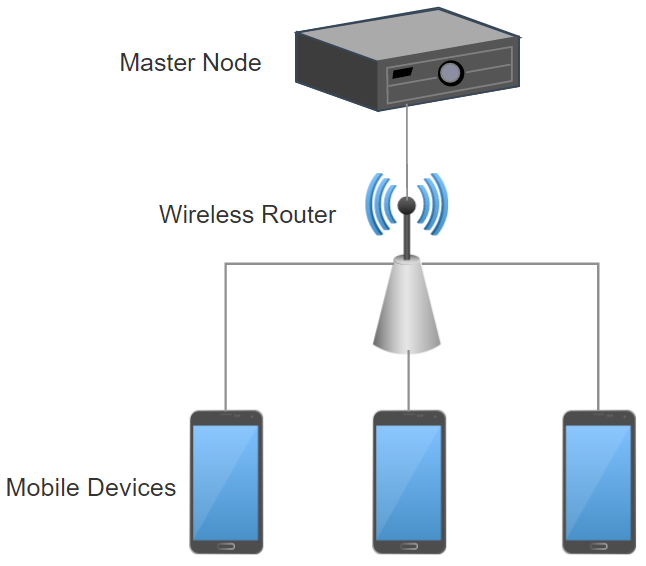
\includegraphics[width=0.8\linewidth]{mstorm_network.png} 
\end{center}	   
\caption{Networking in Actual Mobile Storm Cluster}\label{mstorm_network}
\end{figure}

\begin{figure}[htbp]
\begin{center}
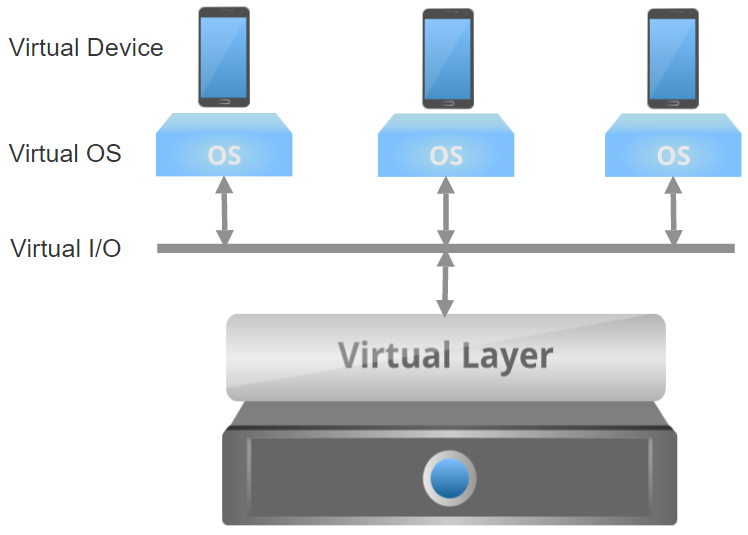
\includegraphics[width=0.8\linewidth]{virtualized_network.png} 
\end{center}	   
\caption{Networking in Virtualized Mobile Storm}\label{virtualized_network}
\end{figure}

\subsection{Existing Solutions}
Though there is a huge trunk of research papers in the field of cloud computing, virtualization as well as mobile clouds, there are few works dedicated to scaling mobile cloud benchmark by virtualizing mobile devices on public clouds, most highly relevant systems are commercialized and available now on market place of AWS. Ravello Systems and Genymotion are two commercial platforms that enable the scalability benchmark for mobile cloud. Ravello Systems enables us to run any virtual machine on any cloud without making any changes through adding a new hypervisor called HVX on top of VMs provided by public cloud platforms. Breaking down the stack of Ravello's solution, as shown in \ref{hvx_diagram}, we can see that we can further run hypervisor on VMs provided by AWS and then run any Virtual Machine on top of the hypervisor. The solutions provided by Genymotion incorporate two aspects, one is to emulate Android x86 OS on top of a host OS in a near-native manner (basically running Android x86 on VirtualBox with all hardware acceleration), the other is to emulate Android OS on demand in public cloud. Genymotion on Demand could similarly provide easy pay-as-you-go Android device virtualization while it's close source and its internal mechanism is rarely discussed. While both solutions can be used for scaling mobile cloud benchmark, none of them can restore the actual wireless network scenario thus cannot guarantee realistic benchmark.
\begin{figure}[htbp]
\begin{center}
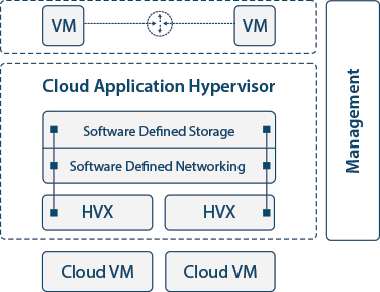
\includegraphics[width=0.8\linewidth]{hvx_diagram.png} 
\end{center}	   
\caption{Destack Ravello System Architecture}\label{hvx_diagram}
\end{figure}

\subsection{Observation and Thoughts}
As shown in Fig. \ref{virtualized_network}, the network of virtual Mobile Storm cluster is based on virtual I/O which is totally different from the wireless network behavior in actual scenario. We assume the virtual I/O is totally reliable. To acquire a wireless-alike environment in the virtualized cluster, our thought is that we might add a router (the router term might not be exactly accurate) on top of virtual I/O to control the traffic. The virtual router is responsible of forwarding data packets to target virtual devices like a wireless link that might generate packet loss, delay, retransmission, basically we wanna incorporate all features of a wireless link as data packets pass through the virtual router.

\subsection{Contribution}
We expect the contributions of this paper as follows:
\begin{itemize}
	\item Propose a new approach of virtualizing mobile cloud directly on top of the Xen virtualization layer, i.e., be able to run android virtual devices cluster on Xen environment, this might also require efforts in virtualized networking as we need to figure out a way for building the interconnectivity between different virtual devices.
	\item Develop a virtual router sitting on top of the virtual I/O to forward data packet and control the transmission between different virtual devices, the final goal of the virtual router is to emulate a wireless network behavior on virtual I/O so that we obtain a realistic environment when virtualizing mobile devices cluster on public clouds.
\end{itemize}

\section{Related Works}
Current solutions for virtualizing mobile devices on cloud mainly include Genymotion  \cite{genymotion} and Ravello Systems. They can both provide pretty good performance for virtualized devices and are highly scalable, but none of them takes common wireless communication paradigms between mobile devices into consideration. This is far from ideal as it is proved in \cite{cen2003end} the wireless network differs a lot from wired network. Both wireless and wired network simulation or emulation have been studied thoroughly in the last decades \cite{zheng2003empower} \cite{judd2005using}. Network virtualization can be realized directly through virtualization systems like VMWare, VirtualBox or Xen, common networking provided by those virtualization systems include NAT, Host-only and bridged. Related works in network virtualization area include \cite{menon2006optimizing} \cite{chowdhury2009network}. However, few researches are dedicated in wireless network emulation in virtualized environment, we need a physical wireless network card on the host machine to acquire wireless behavior for VMs, which is impractical in public cloud. Among all related works, we focus on the following researches as they are the most related ones to our topic:
\subsection{Empower: a network emulator for wireline and wireless networks}
Empower\cite{zheng2003empower} is a distributed network emulation system. It is able to facilitate the emulation of either wireline or wireless networks. In the case when network topology is critical to the underlying network protocol, the emulator could provide specific mechanisms to emulate network topology. Empower can also generate user-defined network conditions and traffic dynamics at packet level.
However,  Empower is specialized in dealing with emulation for wire and wireless networks, which does nothing with cloud service computing. Therefore, we need to move forward for other applications which would fit our concern more.

\subsection{HVX: Virtualizing the Cloud}
HVX \cite{hvx} is a virtualization platform that enables complete abstraction of underlying cloud infrastructure from the application virtual machines. HVX allows deployment of existing VMs into the cloud without any modifications, mobility between the clouds and easy duplication of the entire deployment. HVX can be deployed on almost any existing IaaS cloud. Each instance of the HVX deployment packs in a nested hypervisor, virtual hardware, network and storage configuration. Combined with image store and management APIs, the HVX can be used for the creation of a virtual cloud that utilizes existing cloud provider infrastructure as the hardware rather than using physical servers, switches and storage.However, HVX's virtualization still exhibits the problem that it is unable to simulate the real world wireless communication, which may have higher latency and packets loss rate than wired connection, which HVX adopt at its end.  On the other hand, HVX could be referred as running virtualization on VM, which would significantly slow down the speed. Thus, we may need to propose a better solution to optimize discussed problems. 

\subsection{Genymotion on Demand}
Genymotion \cite{genymotion} is a new cloud-based virtualization platform aimed at Android developers. Running on Amazon Web Services, Genymotion On Demand offers access to the full Android operating environment online. However, Genymotion on Demand is a closed source software whose source code is not published. Therefore, we currently could not be guaranteed whether performance of Genymotion on Demand could satisfy our requirements.

\subsection{Xen}
Xen \cite{barham2003xen} is an x86 virtual machine monitor which allows multiple commodity operating systems to share conventional hardware in a safe and resource managed fashion, but without sacrificing either performance or functionality. This is achieved by providing an idealized virtual machine abstraction to which operating systems such as Linux, BSD and Windows XP, can be ported with minimal effort. The virtualization approach taken by Xen is extremely efficient: it allows operating systems such as Linux and Windows XP to be hosted simultaneously only with a negligible performance overhead --- at most a few percent compared with the unvirtualized case. 

The advantages of virtualization with Xen comparing to other solutions are as follows:
\begin{itemize}
	\item Independence on hardware and the support for different operating systems (both commercial and open source OSs).
	\item Neither performance nor security and functionalities are sacrificed in Xen to accomodate each other.
	\item Xen offers resource isolation and performance guarantees for VMs running on it without risk of DoS.
	\item It is now open sourced as Xen Project \cite{xenproj} in collaboration with Linux Foundation and enjoys technical support from a huge community.
\end{itemize}

Due to those advantages, Xen soon gains popularity with modern public cloud services like AWS. In this paper, we adopt XenServer\cite{xenserver}, an open-source virtualization platform that has been accepted by current industry based on Xen Project hypervisor, as our environment for virtualizing Android devices to build a scalable mobile cloud. We will briefly discuss other available mobile cloud virtualization approaches as well as the XenServer setup we used in our paper in the following sections. 

%Compared with Xen, many other virtualization systems expose a lot of disadvantages. Some require specialized hardware, or cannot support commodity operating systems. Some target $100\%$ binary compatibility at the expense of performance. Others sacrifice security or functionality for speed. Few offer resource isolation or performance guarantees; most provide only best-effort provisioning, risking denial of service. Xen overcomes all above cons, and thus gains popularity with modern public cloud service like AWS. In this paper, we built our virtualized mobile cluster on XenServer, a commercial implementation of Xen. Our research will conducted based on Xen as well. With functions Xen provide, we will further extend and optimize the performance to achieve a faster virtualization environment for real-world wireless cloud service simulation.

\section{Proposed Solution}
\subsection{Virtualizing Mobile Devices in Cloud}
Ravello systems provided solution to run any virtual machine on any cloud without changes to operating systems through nested virtualization, however there will be additional overhead in the 2nd layer of virtualization in terms of processor and memory speed, I/O, network, etc. Moreover, normal customers of public clouds are serviced directly from the virtualized OS level (i.e., an operating system like Windows or Linux is immediately installed per user's request) and they might not have access to nested virtualization as it's a low level setting in Xen which is not commonly exposed by cloud platforms for security considerations. Here in this paper we propose to virtualize Android system directly on top of Xen, which can greatly reduce overheads mentioned above and this is practical as long as Android image is supported in the cloud. More specifically, we use XenServer as the hypervisor for managing resources of the physical machine and install Android directly on VMs without any intermediate Linux or Windows system.

\subsection{Wireless Emulator on Virtual I/O}
As we have mentioned before, we can test the scalibility of a mobile cloud platform easily by leveraging virtualization techniques on public clouds, however, such an approach cannot provide a realistic wireless networking environment as the communication between different virtual devices goes through the virtual I/O, which is either based on system I/O or wired network between different host servers. To better emulate the actual wireless networked mobile cloud platform, we propose a wireless network emulator on top of virtual I/O to virtually control the delivery of data packet between different virtual devices to acquire a network transmission pattern similar to real wireless network system. As shown in Fig. \ref{virtual_router}, the virtual wireless network emulator lies on the virtual I/O layer and is responsible for coordinating the network transmission between different virtual devices. At the current stage, we expect the emulator to be an application on Android, it might exposes some ports to receive and forward data packets in the virtualized network, it works by dropping packets and do retransmission in a wireless manner. 
\begin{figure}[htbp]
\begin{center}
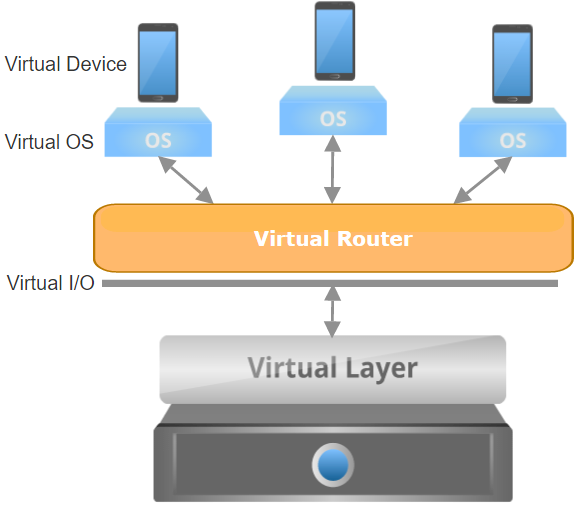
\includegraphics[width=0.8\linewidth]{virtual_router.png} 
\end{center}	   
\caption{Virtual Wireless Network Emulator}\label{virtual_router}
\end{figure}

\subsection{Expected Chanllenges}
Our project is highly challenging in that it incorporates problems in both virtualization and networking, basically we need to find proper approach to achieve the following goals:
\begin{itemize}
	\item Improving virtual device performance: virtual machines are typically much slower than physical machines with the same hardware and software configuration, even with the hardware speedup provided by newly introduced Intel VT-x or AMD-V CPU, which makes the benchmark harder. To reduce the virtualization overhead, we propose to virtualize mobile devices at the lowest level possible and we adopt Android for x86 to acquire better support for desktop CPUs like Intel Core series (oppsed to typical Android device CPU like ARM).
	\item Networking in virtualized environment: as we mentioned above, we need to virtualize mobile device cluster using XenServer, however, to the best of our knowledge so far, native network is not provided directly by the virtualized Android system on XenServer, we might have to deal with device driver and figure out a way to network virtual devices in either the same machine or LAN.
	\item Wireless network emulation: though a huge volume of researches have been put into wireless network emulation and simulation, here we expect many challenges since we are doing emulation on Android platform and the whole system lies in a virtualized environment, the final implementation of wireless emulation should be a totally different story comparing to previous work.
\end{itemize}

\section{Experimental Setup}
To validate our argument that the virtualized networking is totally different from actual wireless environment applied in mobile cloud, we did a series of preliminary experiments to capture the characteristics of virtual network and actual wireless network. In this section we present the setup of our virtualized environment as well as methodologies we adopted in preliminary experiments.
\subsection{XenServer Virtualization Environment}
\subsubsection{Hardware Configuration}
As we have mentioned before, Xen is independent on the underlying hardware and supports various operating systems, however one thing worth mention is that Xen does require a standard 64-bit x86-based system to support paravirtualized linux, a standard 64-bit x86-based system with Intel VT or AMD-V for running Windows. In our case, we failed to virtualize Android system on an  old AMD server (no AMD-V support) but we succeeded in running both Linux and Android on two Intel Core 2 platform (with Intel VT support). Eventually we set up 3 Android VMs across two Intel-based PCs: a Dell OptiPlex 755 PC with Core 2 Duo CPU E8400@3.00GHz and 4GB RAM, running 1 Android instance; a HP DC7900 PC with the same CPU but 8GB RAM, running 2 Android instances. Be noticed that if not otherwise indicated, we use a standard Android instance of the following configurations defaultly:
\begin{itemize}
	\item {\bf Virtual Hardware: }2 vCPUs and 2GB RAM, 8GB internal storage and a Virtual Network Interface.
	\item {\bf System: }Android x86 5.1 Lollipop rc1 (64 bit).
\end{itemize}

The physical Android machines we adopted in the preliminary experiments are two Huawei Y538 smartphones, with Quad-core Snapdragon 210 processor@1.1GHz, 1GB RAM, running Android 5.1.1 (32 bit). The server (referred as master node in mobile cloud) we used is a Y570 laptop with Core i7 CPU and 8GB RAM, running Windows 10.

\subsubsection{Android x86 on XenServer}
One important reason that we choose Android over iOS or other mobile OSs is that Android is an open-source OS with the support from Google and a huge community. However, Android is developed for mobile devices at the first place and it has certain requirements on hardware configurations. Though native Android system runs pretty fast on smartphones and tablets with mostly ARM-based CPUs, it's a nightmare to run it on desktop CPUs like Intel and AMD. In order to speed up Android on desktop

\begin{figure*}
  \centering
  \subfigure[Bridged Networking in VMWare]{
    \label{vmware_bridging} %% label for first subfigure
    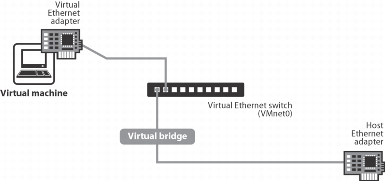
\includegraphics[width=0.45\linewidth]{vmware_bridging.png}}
  \subfigure[NAT Networking in VMWare]{
    \label{vmware_nat} %% label for second subfigure
    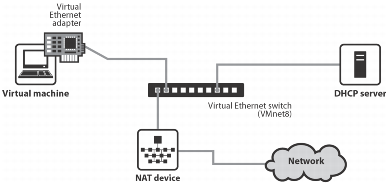
\includegraphics[width=0.45\linewidth]{vmware_nat.png}}
 \subfigure[Host-only Networking in VMWare]{
    \label{vmware_hostonly} %% label for first subfigure
    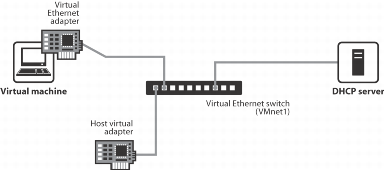
\includegraphics[width=0.45\linewidth]{vmware_hostonly.png}}
  \caption{VMWare/VirtualBox Networking Mechanisms at a Glance}
  \label{vmware_net} %% label for entire figure
\end{figure*}

\noindent hardware, the community have ported Android to x86 platform by modifying the linux kernel and HALs (Hardware Abstraction Layer) of native Android, known as Android x86\cite{android-x86}. It is shown in some benchmarks that Android x86 outperforms native Android by over 100x with similar hardware configurations\cite{android_x86_bench}. For the sake of Android VM performance, we instead adopted Android x86 and installed it on several VMs on XenServer for virtulizing mobile cloud.

\subsubsection{Networking}
Before introducing the network setup in our experiments, we briefly introduce the virtualized network paradigms in existing virtualization systems. The commonly used desktop virtualization solution, VMWare Workstation\cite{vmworkstation} 

\noindent and VirtualBox\cite{vbox}, adopted similar networking mechanisms and they provide 3 solutions for VM networking:

\begin{itemize}
	\item {\bf Bridged: }In bridged networking, a VM will be assigned unique identity on the same external network that the host machine lies in. Take VMWare Workstation as an example, this is achieved by bridging the Virtual Ethernet Switch to the physical Ethernet adapter on host as shown in Figure \ref{vmware_bridging}.
	\item {\bf Network Address Translating (NAT): }VMs configured in NAT mode will form a internal LAN and they share the same network identity with the physical machine. In this case, VM will connect to the virtual Ethernet switch and be assigned an private net IP address by a virtual DHCP server. For access to external network, VM sends packets to the host and the packets will be forwarded after NAT is done. A simple demonstration of the NAT mechanism is shown in Figure \ref{vmware_nat}.
	\item {\bf Host-only: }Host-only mode provides a private network connection between the VM and the host using a similar virtual Ethernet switch, as shown in \ref{vmware_hostonly}. The only difference between Host-only and NAT is that no NAT will be done on the host in Host-only mode.
\end{itemize}

In Xen, every VM has a virtual NIC (Network Interface Controller), all of which are connected to the virtual network controlled by the XenServer host, also be noticed that the virtual network utilities provided by XenServer works like a physical Ethernet segment at layer 2 of the OSI, posing the nonrealistic networking between VMs as we discussed. Network solutions similar to Host-only and Bridging are also provided in Xen, however they are referred differencely as internal network and external network, here in our discussion we focus on those network modes provided in XenServer:
\begin{itemize}
	\item {\bf Internal Networking: }Internal Networking is sometimes also referred to as Single-Server Private Network, in which VIFs (virtual interface) of different VMs are connected by a virtual Ethernet and VMs do not have access to external network.
	\item {\bf External Networking: }The only difference between external networking and internal networking is the accessibility to external network (i.e., under internal networking VMs have the same network accessibility as the host does). This is made available by adding a virtual switch between the virtual Ethernet and the PIF (physical interface). 
\end{itemize} 
An illustrative comparison between two network paradigms in Xen is shown in Figure \ref{xen_net}.

\begin{figure*}
  \centering
  \subfigure[Xen Internal Networking Architecture]{
    \label{xen_internal_net} %% label for first subfigure
    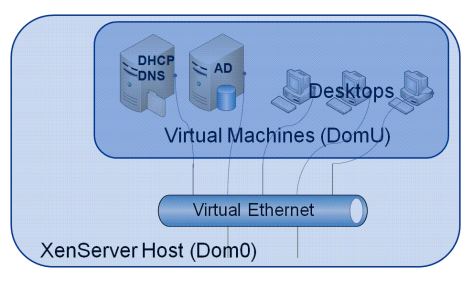
\includegraphics[width=0.45\linewidth]{xen_internal_net.png}}
  \subfigure[Xen External Networking Architecture]{
    \label{xen_external_net} %% label for second subfigure
    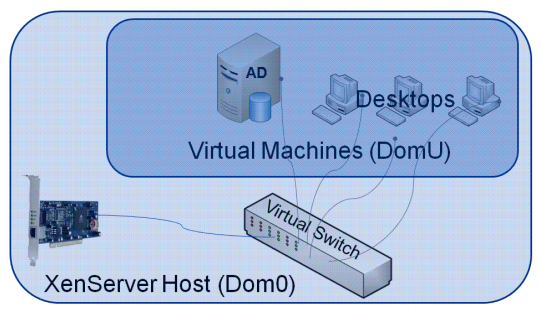
\includegraphics[width=0.45\linewidth]{xen_external_net.png}}
 \subfigure[Xen Routing between Internal Network and External Network]{
    \label{xen_routing} %% label for first subfigure
    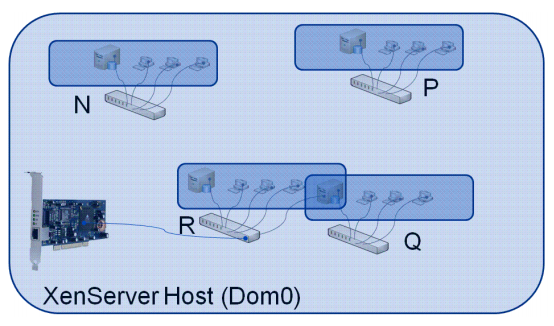
\includegraphics[width=0.45\linewidth]{xen_routing.png}}
  \caption{Xen Networking Mechanisms at a Glance}
  \label{xen_net} %% label for entire figure
\end{figure*}

As our goal in the preliminary experiments is to show the great differences between virtualized network and actual wireless connections between smartphones, we set up two Local Area Networks (LANs) respectively, one as a network connected by a wireless router with a subnet virtualized using XenServer across Android VMs, the other is a simple wireless LAN across master node and physical Android smartphones. 

\begin{figure}[htbp]
\begin{center}
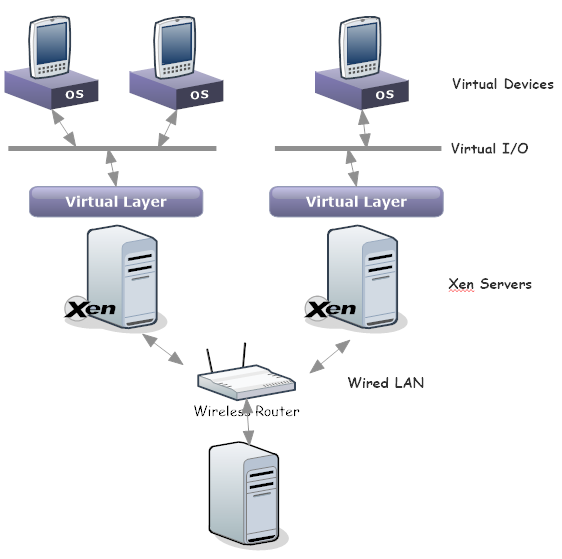
\includegraphics[width=0.8\linewidth]{vnet_arch.png} 
\end{center}	   
\caption{Experimental Setup for Virtualized Mobile Cloud}\label{vnet_arch}
\end{figure}

\begin{itemize}
	\item {\bf Virtualized Networking: }we have two xenservers and the master node connected to a wireless router through wired network, 3 virtual Android devices are virtualized on xenservers thus they are connected to each other either by system I/O or by wired network, a figure that illustrates the system and network architecture in this case is shown in Figure \ref{vnet_arch}.
	\item {\bf Physical Networking: }in experiments of actual wireless networking, we have two Huawei devices connected to the wireless router through WiFi, the master node is again connected to router by wired network as showin in Figure \ref{pnet_arch}.
\end{itemize}

\begin{figure}[htbp]
\begin{center}
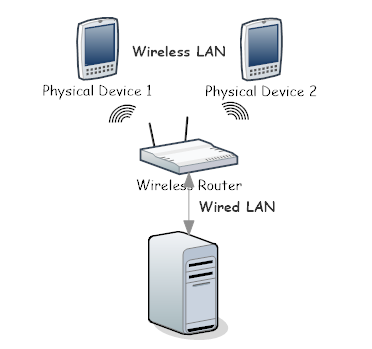
\includegraphics[width=0.8\linewidth]{pnet_arch.png} 
\end{center}	   
\caption{Experimental Setup for Actual Wireless Mobile Cloud Paradigm}\label{pnet_arch}
\end{figure}

\subsection{Benchmarking Network on Android}
To characterize the features of both virtualized network and actual wireless network, we need some proper benchmarks to stress the network and probe important metrics in the data transmission process, in this section we first review the current existing solutions for benchmarking network on Android platform and then propose the methodologies we applied in our experiments.
\subsubsection{Literature Review}
Though Android network benchmarking gains few attentions from the academia, there are a huge trunk of network tools in Google Play to characterize mainly the wireless network performance of Android. Aruba Utilities\cite{aruba_utility} includes a number of tools useful for characterizing and troubleshooting wireless LANs, some of which can work under any WLAN network while others are designed specifically for Aruba products. For our concern, Aruba Utilities has a Wi-Fi monitor
showing the Wi-Fi environment such as current access point, and dynamic signal
strength. It includes Android versions of iPerf\cite{tirumala2005iperf} (a cross-platform tool for active measurements of the maximum achievable bandwidth on IP networks), Ping, DNS and mDNS, which all offer
network test functionality. The measurements are written to a plain-text log file and
various csv report files, which could be saved for later use. JPerf\cite{brethour2003jperf} is a graphical front end for the popular network testing tool iPerf. JPerf provides a quick test for WAN or LAN connection to determine the maximum network throughput. Test results will be automatically graphed and presented in a easy-to-read format. Moreover, it can also be used to detect packet loss, delay, jitter, and other common network problems. Other network tools and speed test APPs include WiFi Speed Test\cite{wifi_test}, which provides real-time monitoring of data transmission speed between specified server and client; he.net\cite{iperf}, developed based on iPerf and provides GUI for network diagnostics, gathering and visualizing network performance/status; etc. However, The above mentioned application are all based on iPerf, except for that they do introduce some new
features like user-friendly GUI (jPerf), IP Calculator (he.net) and
link coverage measurements (Aruba Utilities). A common disadvantage of them is that they by default call Android WifiManager API to set up the network connection and perform  their
tests only under Wi-Fi environment. In our virtualized environment or even in the actual scenario (as Ethernet is also supported in Android), the network for benchmarking doesn't necessarily has to be wireless. Therefore, in the wired network scenarios like virtualized mobile cloud, those APPs can simply crash when trying to setup the connection. To correctly benchmark both the performance of wired and wireless network, we propose to simply port iPerf on Android and execute it at the terminal without any GUI.
\subsubsection{Categorizing Transmissions in Mobile Cloud}
In mobile cloud as shown in \ref{virtualized_network}, we have a master node who serves like a manager of the cluster and the mobile devices are usually referred as slave nodes. Consider centralized task scheduling and task allocation, the most widely used cloud management paradigm, in which the master node collects all heartbeats from slaves and allocates tasks to them based on the current load information of slaves, typical network transmissions in this management scheme can be categorized as follows:
\begin{itemize}
	\item {\bf Master-to-Slave: }a Master-to-Slave transmission happens when the master node transmits scheduling decisions and task input data to slaves through the wireless link. In such transmissions, though the reliability can be guaranteed by using TCP, the instability of wireless link might lead to high latencies in delivering scheduling decisions, low bandwidth would also result in higher response time as the input data cannot be transmitted timely.
	\item {\bf Slave-to-Master: }typical Slave-to-Master transmission includes the regular heartbeat from slave to master node (which is sometimes referred to as status report), in some cases, the execution results might also be returned to master node through the wireless link. Late arrivals of heartbeat might lead to wrong scheduling decisions while delay of returning data lengthens the average response time.
	\item {\bf Slave-to-Slave: }one thing in common among various distributed and cloud computin g platforms is the interaction between different slaves. The intercommunication between those slaves in the cluster can be transmissions for intermediate results, job/task migrations per scheduling requests, etc. 
\end{itemize}
Apparently from the discussions above, the performance of mobile cloud will be greatly influenced by the network. However, in the virtualized mobile cloud, either the highly reliable wired network or virtual I/O between VMs on the same server can correctly reflect the properties of a realistic wireless network. In the next section, we empirically prove this argument and show different characteristics between virtualized and actual wireless network in both 3 types of transmissions mentioned above.

\begin{figure*}
  \centering
  \subfigure[Slave-to-Slave Bandwidth]{
    \label{c_c_bw} %% label for first subfigure
    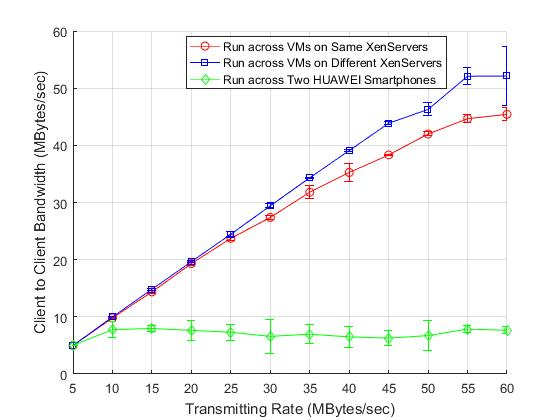
\includegraphics[width=0.32\linewidth]{c_c_bw.jpg}}
  \subfigure[Slave-to-Slave Packet Loss]{
    \label{c_c_pl} %% label for second subfigure
    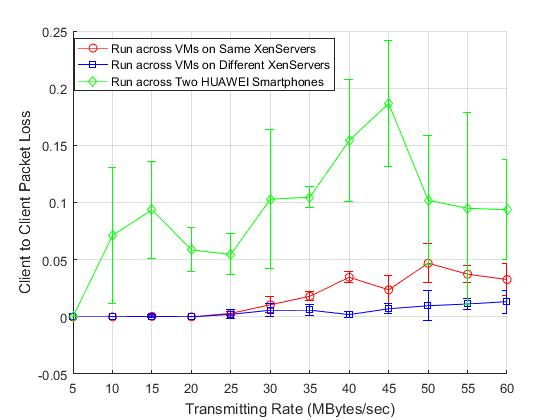
\includegraphics[width=0.32\linewidth]{c_c_pl.jpg}}
 \subfigure[Slave-to-Slave Jitter]{
    \label{c_c_jitter} %% label for first subfigure
    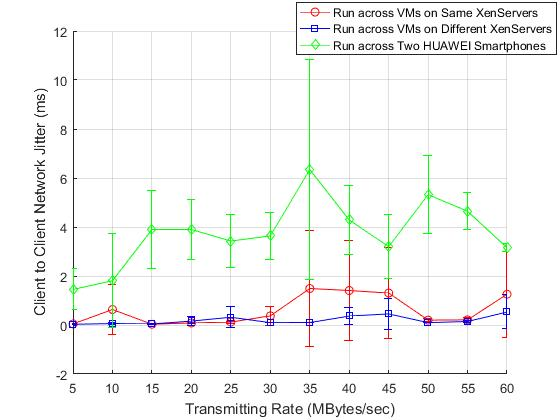
\includegraphics[width=0.32\linewidth]{c_c_jitter.jpg}}
  \caption{Network Characteristics Comparison for Slave-to-Slave Communication}
  \label{c_c} %% label for entire figure
\end{figure*}

\section{Preliminary Observations}
\subsection{Experiment Methodologies}
Recall that the purpose of our experiment is to find out the differences between virtualized and actual wireless network in terms of common network metrics. As discussed in the last section, there are 3 different types of network traffics and we definitely want to characterize them under both virtualized environment and actual environment. We propose to use bandwidth, packet loss and jitter as metrics for describing the network since they might significantly influence the performance of mobile cloud as follows:
\begin{itemize}
	\item {\bf Bandwidth: }the bandwidth of a certain transmission category is important in the sense that it could precisely reflect the long-term performance and capacity of a network, which directly determines the capacity of mobile cloud platform. For example, in distributed stream processing cluster, the system throughput is upper bounded by the bandwidth of the wireless network.
	\item {\bf Packet Loss: }in mobile clouds that adopt unreliable transmission protocols, packet losses of the network directly lead to unreliability of the platform while in other mobile clouds packet losses are the major contributor of network jitters.
	\item {\bf Jitter: }jitters in the network might result in delays of scheduling decisions from the master node, underutilization of downstream computing resources as well as wrong scheduling decisions as mentioned before.
\end{itemize}
A common strategy to probe the network capacity and other characteristics is to gradually stress the network and collect metrics data for analysis. Following the physical and virtual environment settings proposed in section IV, for each transmission category we set the receiver as the iPerf server and the sender as the iPerf client and then stress the network by sending data at a transmitting rate ranging from 5 Mbps to 60 Mbps (5 Mbps as interval) in 10 seconds and record the corresponding metrics we obtain. We conduct experiments in both virtualized and wireless environments and repeat the experiments for 3 times in different time of a day. The final result we acquire is a tendency diagram (increasing transmitting rate) with error bars to mitigate the variance influences and observe fluctuations of network status under different networking scenarios.

\subsection{Slave-to-Slave Network Characteristics}
The metrics we measured under different traffic load for Slave-to-Slave transmissions are shown in Figure \ref{c_c}. Be noticed that this test differs from all other experiments in that we have three groups of data for comparison. The underlying reason is that for Slave-to-Slave transmission in virtualized environment, we also have two scenarios:
\begin{itemize}
	\item Data transmissions happening between VMs across different XenServer.
	\item Data transmissions happening between VMs on the same XenServer.
\end{itemize}
From the bandwidth tendency shown in Figure \ref{c_c_bw}, we can see that at the very beginning, the bandwidth of all three scenarios increases with the transmitting rate. However, immediately as the transmitting rate exceeds 5 Mbps the actual wireless network seems to be overloaded and the following bandwidth (no matter how much the transmitting rate increases) stay around 8 Mbps. For both other two kinds of network, their maximum bandwidth is much higher than the actual scenarios. Internal VM network and across-server VM network respectively yields maximum bandwidth around 45 Mbps and 52 Mbps. Furthermore, by analyzing jitters and packet losses, we can also get a basic understanding of the high unstability in wireless network comparing to its counterparts. For short, the wireless link in the actual scenario yields much lower bandwidth, produces a lot more jitters and packet losses, and is highly unstable.

\begin{figure*}
  \centering
  \subfigure[Master-to-Slave Bandwidth]{
    \label{s_c_bw} %% label for first subfigure
    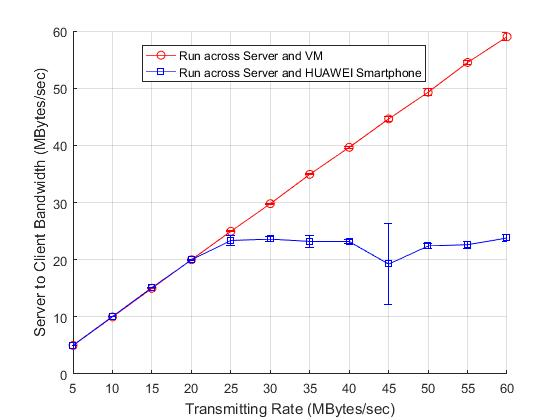
\includegraphics[width=0.32\linewidth]{s_c_bw.jpg}}
  \subfigure[Master-to-Slave Packet Loss]{
    \label{s_c_pl} %% label for second subfigure
    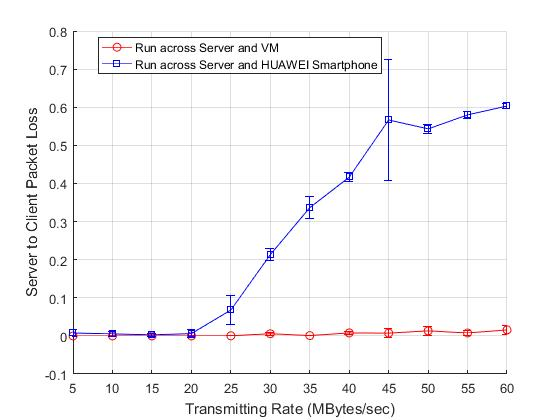
\includegraphics[width=0.32\linewidth]{s_c_pl.jpg}}
 \subfigure[Master-to-Slave Jitter]{
    \label{s_c_jitter} %% label for first subfigure
    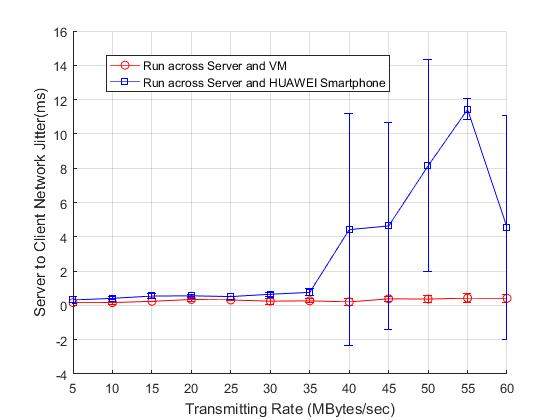
\includegraphics[width=0.32\linewidth]{s_c_jitter.jpg}}
  \caption{Network Characteristics Comparison for Master-to-Slave Communication}
  \label{s_c} %% label for entire figure
\end{figure*}

\begin{figure*}
  \centering
  \subfigure[Slave-to-Master Bandwidth]{
    \label{c_s_bw} %% label for first subfigure
    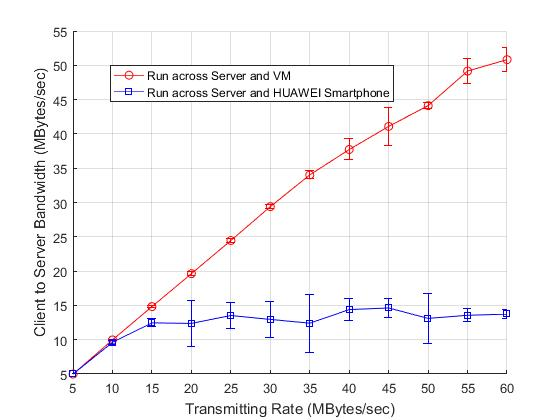
\includegraphics[width=0.32\linewidth]{c_s_bw.jpg}}
  \subfigure[Slave-to-Master Packet Loss]{
    \label{c_s_pl} %% label for second subfigure
    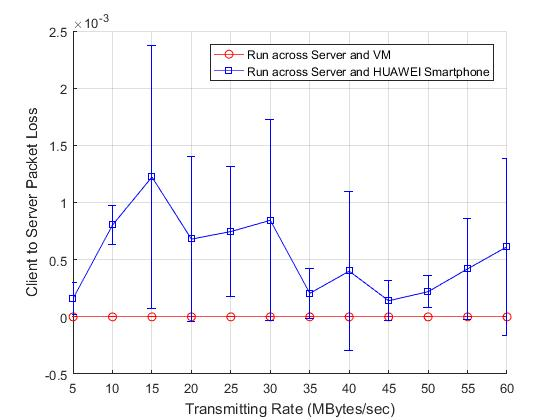
\includegraphics[width=0.32\linewidth]{c_s_pl.jpg}}
 \subfigure[Slave-to-Master Jitter]{
    \label{c_s_jitter} %% label for first subfigure
    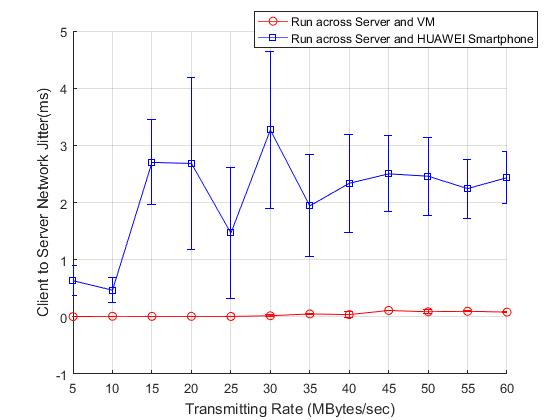
\includegraphics[width=0.32\linewidth]{c_s_jitter.jpg}}
  \caption{Network Characteristics Comparison for Slave-to-Master Communication}
  \label{c_s} %% label for entire figure
\end{figure*}

\subsection{Master-to-Slave Network Characteristics}
The metrics we measured under different traffic load for Master-to-Slave transmissions are shown in Figure \ref{s_c}. Apparently the figure shows a much better bandwidth for actual Master-to-Slave network, around 25 Mbps, this makes sense due to the fact that only one device is occupying the wireless channel in this scenario which means much less interferences, collisions and backoffs. However, we also noticed the increasingly high packet loss rate and jitters in this experiment are due to overloading of wireless link, while currently we cannot find a proper explanation for why both packet losses and jitters in this scenario exceed the Slave-to-Slave case. Again, the wireless link is highly unstable if we look at the error bars.

\subsection{Slave-to-Master Network Characteristics}
The metrics we measured under different traffic load for Slave-to-Master transmissions are shown in Figure \ref{c_s}. Through the measurement figures, we can see that the results look similar to the Slave-to-Slave case. The only one thing worth mention here is that the Slave-to-Master bandwidth lies in between the max bandwidth of Master-to-Slave and Slave-to-Slave. On the one hand, we don't have much interferences in this case, therefore we can transmit data faster than Slave-to-Slave. On the other hand, it's common for an actual wireless router to have lower uplink bandwidth than downlink, thus the network performance here is inferior to the Master-to-Server case.

\section{Characterizing and Emulating Wireless Network}
\subsection{Characterizing Wireless Features}

\subsection{Shaping Virtualized Network}

\section{Experiments}
\subsection{Distribution}
3 types of distributions when doing experiments:
1. m to s
2. s to m
3. s to s
for each of the distribution, we do iperf and ping experiments after setting the distribution

TODO:
1. how to determine the tc params for getting best-fit packet loss curve

assuming we have a script for automated testing, it repetitively test iperf metrics and ping metrics
this is the manual of tc:
http://man7.org/linux/man-pages/man8/tc-netem.8.html

Steps for doing experiments:
distributions we need:
1. c2c, redo
2. c2s
3. s2c
find a way to get the distribution drew as a graph, hopefully we can get a normal distribution?
graph 1


1. DO NOT apply distribution now, first reevaluate the original network pattern, be noticed that this includes all the experiments we did in last including both the virtualized env and the real env, also including the two cases for c2c: vm across server and on the same server
	1.1. use iperf_bat_android.sh for testing both c2c, s2c, c2s traffic, notice that we should change  some of the codes for different devices, check all TODOs in the script to see what should be changed
	1.2. use ping command to test the delay (rtt) of both virtualized case and actual case, draw the delay distribution graph
	
2. apply distribution respectively, every time a distribution is applied test the corresponding scenario
	1.1. how to apply distribution

\subsection{Bandwidth}
Use iperf to test the bandwidth, this shall be the simplest for emulation.

\subsection{Delay}
distribution figure
Use ping command to test the delay of both virtualized network with emulation. We should get very good results here. 

\subsection{Packet Loss}
Use iperf. 

\subsection{Jitter}
Use iperf. 

\section{Conclusion}
So far in this paper, we have established two mobile cloud systems, one based on efficient direct virtualization while the other is an actual mobile cloud connected through wireless link. A detailed review and analysis of networking in virtualized environment are also provided.  For network benchmarking, iPerf 2 is poted to Android platform and several tricks are applied before it executes successfully. The major contribution of our paper by now is an empirical analysis of network differences between virtualized and actual wireless scenario. Through a series of experiments, we have shown that virtualized environment is nonrealistic for testing mobile clouds since it enjoys much higher bandwidth and is really stable in terms of jitter and packet losses, comparing to a common wireless link.

\section{Future Work}
\subsection{Bridging Wireless to Ethernet}
As we have already covered in the literature review of network benchmarking tools on Android, most of those APPs are based purely on WiFi connection due to the dominance of it on mobile devices. This exposes a major problem in our virtualization approach for scaling mobile cloud tests. Most APPs available on Android platforms are like those tools and Ethernet connection adopted in our virtualization approach is not commonly supported. Therefore, we propose to bridge the wireless network interface (wlan0) of virtualized Android system to the Ethernet interface (eth0) so that the wireless traffic can be automatically forwarded to Ethernet. In this way, we will be able to run almost all applications or mobile cloud platforms without any changes and the compatibility of our method will be greatly improved.

\subsection{More Reliable Experiments}
For compatibility considerations, the preliminary experiments are conducted based on iPerf 2.0.5, an obsolete version that is no longer maintained by developers. We discovered several problems in this version of iPerf like we cannot set transmitting rate in MBytes and the TCP-related utilities are limited. We expect to port newer iPerf 3 into experiments which incorporates more functionalities and could be used to capture more features of  the network. Also, currently we are testing the network in an environment with many interferences, we expect a great probability that the uncommonly high packet losses and jitters in Figure \ref{s_c} are caused by those interferences. Additionally, though repeated experiments are carried out, we are still looking for new methodologies that involves a lot more tests for recognizing the wireless network performance pattern.

\subsection{Characterizing and Emulating Wireless Network}
We expect a large amount of long-term and short-term experiments in the future so that we might be able to capture the bandwidth/jitters/packet losses distribution of wireless link and find a way to emulate it in virtualized environment.
% Can use something like this to put references on a page
% by themselves when using endfloat and the captionsoff option.
\ifCLASSOPTIONcaptionsoff
  \newpage
\fi



% trigger a \newpage just before the given reference
% number - used to balance the columns on the last page
% adjust value as needed - may need to be readjusted if
% the document is modified later
%\IEEEtriggeratref{8}
% The "triggered" command can be changed if desired:
%\IEEEtriggercmd{\enlargethispage{-5in}}

% references section

% can use a bibliography generated by BibTeX as a .bbl file
% BibTeX documentation can be easily obtained at:
% http://mirror.ctan.org/biblio/bibtex/contrib/doc/
% The IEEEtran BibTeX style support page is at:
% http://www.michaelshell.org/tex/ieeetran/bibtex/
%\bibliographystyle{IEEEtran}
% argument is your BibTeX string definitions and bibliography database(s)
%\bibliography{IEEEabrv,../bib/paper}
%
% <OR> manually copy in the resultant .bbl file
% set second argument of \begin to the number of references
% (used to reserve space for the reference number labels box)
\bibliographystyle{IEEEtran}
% argument is your BibTeX string definitions and bibliography database(s)
\bibliography{refs}

% biography section
% 
% If you have an EPS/PDF photo (graphicx package needed) extra braces are
% needed around the contents of the optional argument to biography to prevent
% the LaTeX parser from getting confused when it sees the complicated
% \includegraphics command within an optional argument. (You could create
% your own custom macro containing the \includegraphics command to make things
% simpler here.)
%\begin{IEEEbiography}[{\includegraphics[width=1in,height=1.25in,clip,keepaspectratio]{mshell}}]{Michael Shell}
% or if you just want to reserve a space for a photo:

% that's all folks
\end{document}


